\chapter{Prehľad~problematiky}\label{ch:terminology}

...

\section{Teória~grafov}\label{sec:graph-theory}

Teória grafov je rozsiahla a komplexná oblasť matematiky a informatiky. V tejto kapitole sa zameriame na základné 
pojmy, definície a koncepty, ktoré sú nevyhnutné na pochopenie práce s grafmi, ich vlastností a rôznych aplikácií. 
Pre podrobnejšie informácie a hlbšie pochopenie odporúčam odbornú literatúru, najmä publikáciu
\textit{Graph Theory Fifth Edition od R. Diestela} \cite{diestel2017graph}.

Graf $G$ je reprezentovaný ako dvojica $G = (V, E)$, pričom $V$ \textit{(z angl. vertices)} je množina všetkých
vrcholov a $E$ je množina všetych hrán \textit{(z angl. edges)}, ktoré tvoria spojenia medzi týmito vrcholmi.
Vrcholy grafu sa taktiež nazývajú aj uzly.

Medzi dvojicou vrcholov grafu môže, ale nemusí existovať hrana. Ak medzi nimi hrana existuje, hovoríme, že sú
navzájom prepojené. Jednotlivé hrany, ktoré obsahuje množina $E$, sú reprezentované ako dvojice vrcholov $(u, v)$, 
pričom $u$ a $v$ sú vrcholy z množiny $V$. 

Hrany rozlišujeme na niekoľko typov. Ak má hrana grafu daný smer, nazýva sa orientovaná a záleží
na poradí vrcholov v usporiadanej dvojici, prvý vrchol dvojice predstavuje uzol, od ktorého hrana vychádza a 
druhý vrchol dvojice predstavuje uzol, do ktorého hrana smeruje. Ak hrana nemá určený smer, tak sa jedná o 
neorientovanú hranu a poradie vrcholov v usporiadanej dvojici nie je dôležité. Hranu, ktorá má začiatok a koniec 
v rovnakom vrchole, nazývame slučka. Pojem viacnásobná hrana označuje prípad, kedy medzi dvoma vrcholmi existuje viac ako jedna hrana. 
Rôzne typy hrán je možné vidieť na ilustračnom obrázku č. \ref{obr:edges}.

\begin{figure}
    \centerline{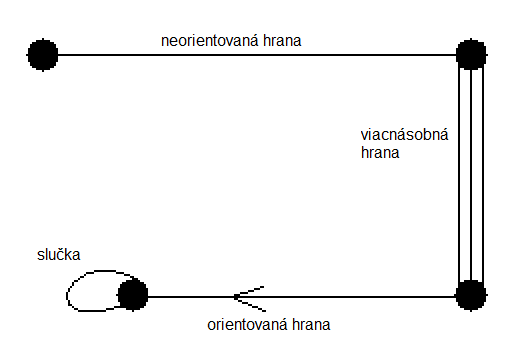
\includegraphics[width=0.5\textwidth]{images/edges.png}}
    \caption[Zobrazenie typov hrán v grafe.]{Zobrazenie typov hrán v grafe.}
    \label{obr:edges}
\end{figure}

Hrany, ktoré majú priradenú číselnú hodnotu, nazývame vážené hrany. Tieto váhy môžu reprezentovať rôzne vlastnosti hrany, 
ako napríklad vzdialenosť medzi vrcholmi alebo náklady na prechod medzi nimi. Sú využívané hlavne v praktických aplikáciách,
ako napríklad dopravné siete.

Pojem jednoduchý graf nám definuje taký graf, ktorý neobsahuje slučky ani viacnásobné hrany. Jednoduchý graf, ktorý neobsahuje 
orientované hrany a vrcholy sú poprepájané spôsobom každý s každým nazývame kompletný graf\cite{markovsovadynamika}.

Pri analýze grafov je treba poznať rôzne spôsoby, akými môžeme prechádzať cez vrcholy a hrany grafu.
Prechod grafom, pri ktorom sa striedajú vrcholy a hrany, ktoré sa môžu opakovať, sa nazýva sled.
Formálny zápis pre sled v grafe $G = (V, E)$ je postupnosť 
\[
v_0, e_0, v_1, e_1, \dots, e_{k-1}, v_{k},
\]
kde $v_i \in V(G)$ pre všetky $i \in \{0, 1, \dots, k\}$ a $e_j \in E(G)$ pre všetky $j \in \{0, 1, \dots, k-1\}$ s podmienkou
$e_i = (v_i, v_{i+1})$. Ťah je špeciálny typ sledu, pri ktorom sa hrany nemôžu opakovať, teda pre všetky $i \neq j$ platí $e_i \neq e_j$.
Vrcholy sa v ťahu môžu opakovať. Sled a ťah majú špeciálny prípad, kedy sa počiatočný a koncový vrchol zhodujú, teda $v_0 = v_k$.
Takýto sled sa nazýva uzavretý sled a ťah uzavretý ťah. Ešte existuje pojem cesta, ktorý predstavuje prechod grafom, pri ktorom sa
nemôžu opakovať ani vrcholy ani hrany.

Spojitý graf je taký graf, v ktorom existuje cesta medzi každými dvoma vrcholmi. Nie každý graf je spojitý, pretože niektoré grafy sa
skladajú z viacerých disjunktných častí, ktoré nie sú navzájom prepojené hranou, teda medzi nimi neexistuje žiadna cesta. Takýmto
disjunktným častiam grafu hovoríme komponenty. Graf s viacero komponentami je nespojitý graf.

Grafy sa dajú reprezentovať rôznymi spôsobmi. Najčastejšia matematická reprezentácia je pomocou matice susedností a matice incidencie.
Nech $G = (V, E)$ je graf s $n = |V|$ vrcholmi a $m = |E|$ hranami. Matica susedností $A$ je $n \times n$ matica, kde každý prvok $a_{ij}$
predstavuje počet hrán medzi vrcholmi $v_i$ a $u_j$. Incidenčná matica $B$ je $n \times m$ matica, kde pre každý prvok platí $b_{ij} = 1$,
ak je hrana $e_j$ incidentná s vrcholom $v_i$, inak $b_{ij} = 0$.
Príklad matice susedností a incidenčnej matice spolu s ilustračným grafom je zobrazený na obrázku č. \ref{obr:matrices}.

\begin{figure}
    \centerline{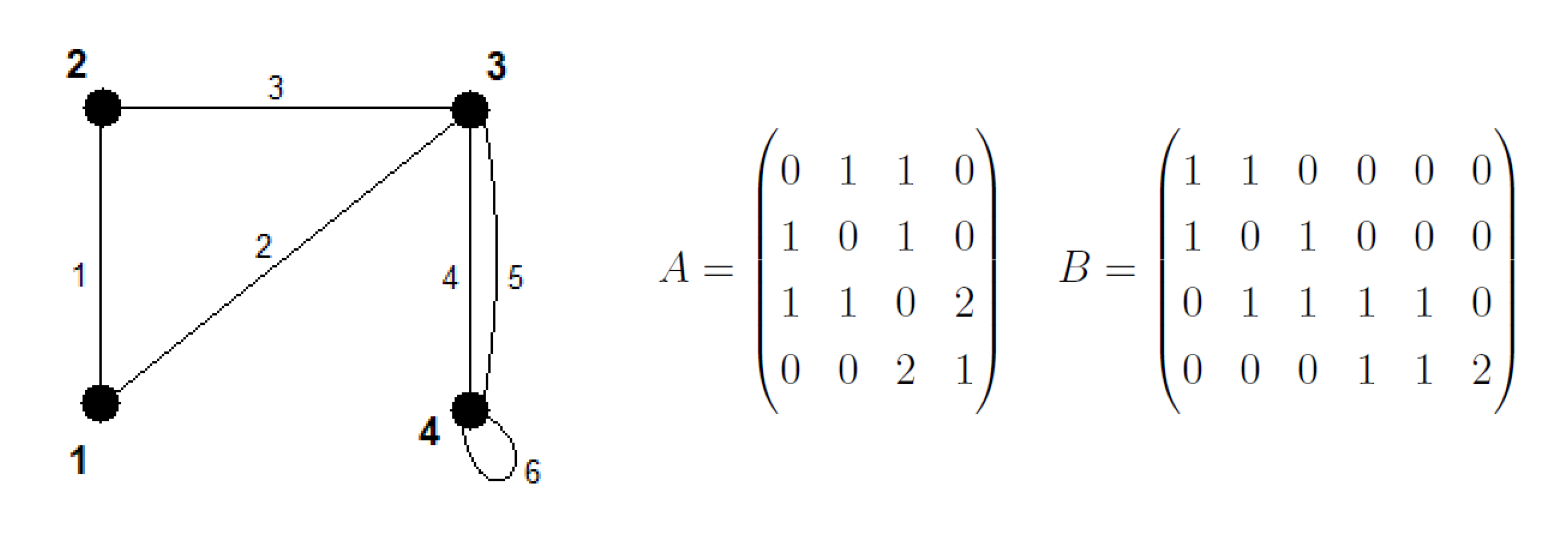
\includegraphics[width=0.8\textwidth]{images/matrices.png}}
    \caption[Matica susedností a incidenčná matica.]{Matica susedností a incidenčná matica pre zobrazený graf.}
    \label{obr:matrices}
\end{figure}

Teraz si predstavíme niekoľko základných vlastností, s ktorými budeme pracovať, ich definície z teórií grafov a ich aplikáciu. Budeme sa zaoberať iba
jednoduchými, neorientovanými grafmi, ak nebude uvedené inak.

Jedna zo základných vlastností vrchola grafu je jeho stupeň. Stupeň vrchola $v$ označovaný aj ako $deg(v)$ nám udáva počet hrán,
ktoré sú incidentné s vrcholom $v$. Minimálna hodnota stupňa vrchola je $0$, vtedy tvorí vrchol samostatný komponent, taktiež sa
nazýva izolovaný vrchol. Maximálna hodnota stupňa vrchola je $n-1$, nastáva keď vrchol susedí s každým vrcholom grafu.
Celkový počet hrán v grafe potom získame ako polovicu súčtu všetkých stupňov vrcholov grafu,
pretože každá hrana je incidentná s dvoma vrcholmi. Tento vzťah môžeme zapísať ako:
\begin{equation}
    L = \frac{1}{2} \sum_{i=1}^{n} deg(v_i),
    \label{eq:pocet_hran}
\end{equation}
kde $L$ predstavuje počet hrán v grafe a $n$ je počet vrcholov\cite{barabasi2016network}.

Taktiež často používanou charakteristikou grafu je priemerný stupeň uzla:
\begin{equation}
    \bar{d} = \frac{1}{n} \sum_{i=1}^{n} deg(v_i) = \frac{2L}{n},
    \label{eq:priemerny_stupen}
\end{equation}
kde $\bar{d}$ je priemerný stupeň uzla a $n$ je počet vrcholov grafu\cite{barabasi2016network}.

Hustota grafu nám určuje, ako blízko je graf ku kompletnému, teda akú časť z maximálneho počtu hrán obsahuje.
Nadobúda hodnoty v intervale $[0, 1]$, pričom $0$ znamená, že graf je prázdny a $1$ znamená, že graf je kompletný.
Formálny zápis pre hustotu grafu je:
\begin{equation}
    D = \frac{2L}{n(n-1)},
    \label{eq:hustota}
\end{equation}
kde $D$ je hustota grafu, $L$ je počet hrán a $n$ je počet vrcholov.

Ďalšou vlastnosťou grafu je koeficient zhlukovania, inak známy aj ako klasterizačný koeficient.
Tento koeficient udáva ako veľmi sú prepojené susedné vrcholy uzla. Hodnota koeficientu sa pohybuje v intervale $[0, 1]$,
kde $0$ značí, že medzi susedmi vrcholu neexistujú žiadne hrany a $1$ znamená, že všetci susedia sú medzi sebou navzájom prepojení.
Nech $v$ je vrchol grafu a $deg(v)$ je jeho stupeň, potom:
\begin{equation}
    C_v = \frac{2L_v}{deg(v)(deg(v)-1)},
    \label{eq:koeficient_zhlukovania_local}
\end{equation}
kde $C_v$ je koeficient zhlukovania vrchola $v$, $L_v$ predstavuje počet hrán medzi $deg(v)$ susedmi vrchola $v$. 
Týmto spôsobom vieme získať lokálny koeficient zhlukovania pre každý vrchol grafu, z ktorých potom vieme vypočítať
priemerný koeficient zhlukovania pre celý graf:
\begin{equation}
    C = \frac{1}{n} \sum_{i=1}^{n} C_{v_i},
    \label{eq:koeficient_zhlukovania_global}
\end{equation}
kde $C$ je priemerný koeficient zhlukovania grafu a $n$ je počet vrcholov grafu\cite{barabasi2016network}.

Pojem najkratšia cesta v grafe nám definuje takú cestu, ktorá spája dva vrcholy grafu a obsahuje najmenší možný počet
hrán. Priemerná najkratšia cesta medzi dvoma vrcholmi je definovaná ako priemer všetkých najkratších ciest medzi
všetkými kombináciami dvojíc vrcholov grafu.	
\begin{equation}
    \ell = \frac{1}{n(n - 1)} \sum_{\substack{i,j = 1 \\ i \ne j}}^{n} d(v_i, v_j),
    \label{eq:avg_shortest_path}
\end{equation}
kde $\ell$ je priemerná najkratšia cesta, $d(v_i, v_j)$ je dĺžka najkratšej cesty medzi vrcholmi $v_i$ a $v_j$ a $n$ je počet vrcholov grafu\cite{barabasi2016network}.

Priemer grafu nám udáva najväčšiu dĺžku najkratšej cesty medzi dvoma rôznymi vrcholmi grafu.
\begin{equation}
    diam = \max_{i \ne j} d(v_i, v_j),
    \label{eq:diameter}
\end{equation}

Veľmi dôležitým parametrom pri analýze grafu je distribúcia stupňov vrcholov, značené ako $p_k$.
Poskytuje pravdepodobnosť, že náhodne vybraný vrchol grafu má práve $k$ susedov\cite{barabasi2016network}.
Pre graf s počtom vrcholov $n$ a počtom vrcholov s $k$ susedmi $n_k$ je distribúcia stupňov definovaná ako:
\begin{equation}
    p_k = \frac{n_k}{n},
    \label{eq:degree_distribution}
\end{equation}
kde $p_k$ je distribúcia stupňov, $n_k$ je počet vrcholov s $k$ susedmi, $n$ je počet vrcholov grafu.

\section{Modely~sietí}\label{sec:network-models}

\subsection{Náhodná~sieť}\label{sec:random-network}

\subsection{Bezškálová~sieť}\label{sec:scale-free-network}

\subsection{Dorogovtsev~Goltsev~Mendes model}\label{sec:dgm-model}

\section{Slovné~siete}\label{sec:word-networks}

Slovné siete predstavujú efektívny spôsob reprezentácie a analýzy jazyka a jeho štruktúry za pomoci teórie grafov.
V takýchto sieťach sú jednotlivé slová reprezentované ako uzly a vzťahy medzi slovami, ktoré sa navzájom ovplyvňujú alebo súvisia
tvoria hrany\cite{motter2002topology}. Podľa metód reprezentácie vzťahov medzi slovami dokážeme slovné siete rozlišovať.
V sémantických slovných sieťach vznikajú prepojenia medzi slovami na základe ich významovej podobnosti. Narozdiel od sémantických
slovných sietí, v syntaktických slovných sieťach sú interakcie medzi slovami založené na slovnej štruktúre a gramatických pravidlách.

Špecifický typ slovnej siete, ktorej sa budeme venovať v tejto práci sa nazýva pozičná slovná sieť. Táto sieť je zameraná na štruktúru
a pozície slov v texte. V pozičnej slovnej sieti uzly tvoria jednotlivé slová a hrany sú vytvorené na základe toho, či sa slová nachádzajú
vedľa seba v texte, susedia. Ukážku takejto siete vidíme na obrázku č. \ref{obr:wan}.

Tieto siete majú niekoľko zaujímavých vlastností. Koeficient zhlukovania, ktorý nám určuje, do akej
miery slová tvoria skupiny alebo často používané frázy. Distribúcia stupňov uzlov, ktorá sa často podobá na rozdelenie 
typu mocninného zákona, čo znamená, že väčšina slov má veľmi nízky stupeň, zatiaľ čo malý podiel slov má veľmi vysoký stupeň\cite{dorogovtsev2001language}.
Toto rozdelenie je typické pre bezškálové siete. Na obrázku č. \ref{obr:degdist} je zobrazená distribúcia stupňov uzlov s dvomi
rôznymi priemernými exponentami $y = -1.5$ a $y = -2.7$. Exponent $y = -2.7$ sa blíži k exponentu pre Barabási-Albertov model, ktorý je
$y_{BA} = -3$\cite{cancho2001small}.

\begin{figure}
    \centerline{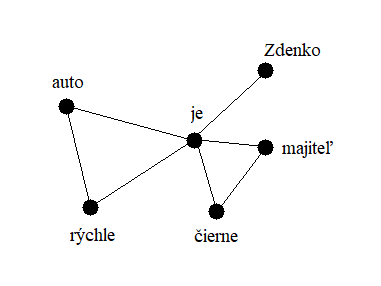
\includegraphics[width=0.8\textwidth]{images/wan.png}}
    \caption[Pozičná slovná sieť.]{Pozičná slovná sieť z viet: „Auto je rýchle. Auto je čierne. Majiteľ je Zdenko.“.}
    \label{obr:wan}
\end{figure}

\begin{figure}
    \centerline{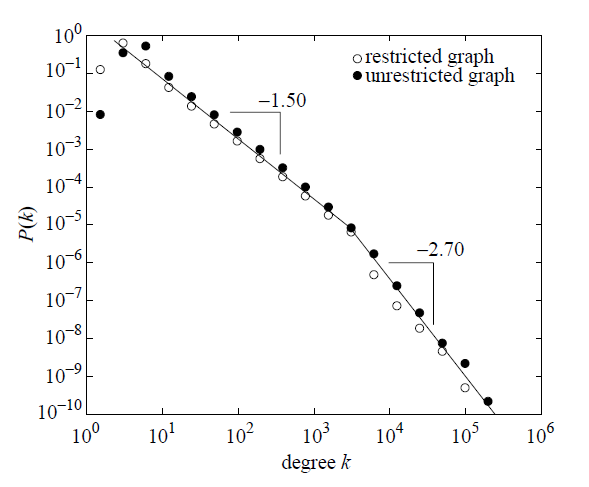
\includegraphics[width=0.8\textwidth]{images/degdist.png}}
    \caption[Distribúcia stupňov vrcholov.]{Distribúcia stupňov vrcholov pre dve siete, body zoskupené mocninou dvoch\cite{cancho2001small}.}
    \label{obr:degdist}
\end{figure}

\clearpage

\section{NetworkX}\label{sec:networkx}

Text ohľadom knižnice NetworkX.